% Generated by uscribe -- do not edit by hand
\documentclass[letterpaper,12pt]{article}
\usepackage[T1]{fontenc}
\usepackage[utf8]{inputenc}
\usepackage{graphicx}
\usepackage{hyperref}
\usepackage{xcolor}
\usepackage{fancyvrb}
\usepackage{booktabs}
\usepackage{longtable}
\usepackage{multirow}
\hypersetup{colorlinks=true,linkcolor=blue,urlcolor=blue}
\begin{document}
\begin{titlepage}
\null\vfil\vskip 40pt
\begin{center}
{\LARGE\bfseries An IVIB Primer \par}
\vskip 3em
{\large\bfseries Susie Jeffery and Clinton Jeffery \par}
\vskip 1.0em
{\bfseries Unicon Technical Report: 6c\par}
\vskip 1.0em
{\large\bfseries 2019-02-28\par}
\vskip 5.5em
{\bfseries Abstract}\par
\begin{quote}
Unicon's improved visual interface builder program IVIB offers many more types of widgets than its precursor, VIB. IVIB also supports colors and fonts, allowing the programmer a wider variety of appearances. This primer explains the rudiments of using IVIB Version 2.
\end{quote}
\vskip 0.8in
{\large\bfseries
Unicon Project\\
\url{http://unicon.org}\\
\ \
University of Idaho\\
Department of Computer Science\\
Moscow, ID, 83844, USA
}
\end{center}
\vfil\null
\end{titlepage}
\setcounter{page}{1}
\section{Introduction}
\label{utr6-introduction}

Most applications these days provide easy to use, graphical interfaces. For the Unicon programmer, several options are available to create such an interface. One option is to use the graphics facilities described in the book "Graphics Programming in Icon" [Gris98]. The Icon Graphics book includes chapters on writing user interfaces using the vidgets library and its interface builder, VIB. Unfortunately, these facilities are hard to customize, either with new widgets or with attributes such as colors or fonts. Another option for MS Windows programmers is to write an interface using MS Windows native facilities available from Icon; they are documented in Icon Project Document 271, but are very limited.


This report describes how to use Unicon's new GUI toolkit and its interface builder program, IVIB. This package was written by Robert Parlett, with minor improvements by the authors and other contributors. Compared with the Icon-based tools, Mr. Parlett's toolkit is elegant, feature-rich, extensible, and deep. Unless you are familiar with similar class libraries, IVIB and its GUI toolkit may seem daunting in its complexity. This report demystifies some typical uses of IVIB Version 2. We hope you come to enjoy it as much as we have. A great deal of additional documentation on these tools can be found in the book "Programming with Unicon" [Jeff01].

\subsection{\emph{Part I     A Simple IVIB Application}}
\label{utr6-part-i-a-simple-ivib-application}
\subsubsection{Hello, Ivib}
\label{utr6-hello-ivib}

Before we delve into a real application, let us create a rhetorical program with a single button that executes a procedure when we click on it. For the sake of tradition, let's suppose our procedure \texttt{p()} is as follows. Go ahead and type this procedure in using the ui program or your favorite text editor, and save it to a file named \texttt{p.icn}.

\begin{Verbatim}[fontsize=\small,frame=single,commandchars=\\\{\}]

procedure p()
   write("hello, world")
end
\end{Verbatim}


To start building our GUI, execute the Ivib program. Below its title bar it has a menu bar with File, Canvas, Selection, and Objects menus, and below that it has a tool bar that allows you to easily create many kinds of widget in the GUI library. Below the toolbar is the main Ivib drawing area, called the canvas.


The Button widget is the top leftmost widget in the toolbar. Go ahead and click on it; a button labeled "Button" appears in the upper left area of the canvas. You can drag it approximately to the center of your canvas area. To modify aspects of the widget's functionality or appearance, right click on it and select Dialog from the popup menu. The widget's setup dialog allows you to change all aspects of the widget. The top half of the dialog controls properties relevant to all widgets, such as position on screen, graphical attributes, and what variable name will hold the widget. The bottom half of the dialog controls properties specific to the particular type of widget being modified (in this case, a TextButton). TextButtons have a Label attribute that contains the text on the face of the button. Click in that text area and change "Button" to "Go!". Then click on the Okay button at the bottom of the dialog. Your resulting screen might look something like this:


Figure 1: go.icn


At this point, you have created a graphical interface with a button on it. When you save this as \texttt{go.icn}, Ivib will generate the Unicon source code for the graphical interface, with the Ivib representation of that graphical interface encoded as a strange looking comment at the end of the file. If you compile it, you can produce a working program, but it won't do anything when the Go! button is pressed.

\subsubsection{Ivib and Event-driven Programming}
\label{utr6-ivib-and-event-driven-programming}

Event-driven programming is writing code in terms of responses to events. You don't own the control flow, the GUI library does. The GUI library calls certain methods in response to each event; your options are to either stick your application code directly in those method bodies, or stick calls to your code in those method bodies.


Suppose our procedure \texttt{p()} given above is located in a file \texttt{p.icn}, which will hopefully be true by now. What we want to do is make the interface call \texttt{p()} whenever the button is pressed. An object (whose class is a subclass of Dialog in package gui) owns the control flow and processes user input. Each user activity (key press, mouse click) in the dialog is turned into an Event object and sent to the interface object being manipulated (the button, scrollbar, or other widget that was "clicked"). In Ivib, the object's dialog has an Events... tab that allows the programmer to associate a different handler method with code to handle each kind of event. To sum up: an interface has a corresponding Dialog class. For each widget \emph{foo} you can optionally ask for a class variable \texttt{foo} that holds the actual widget object reference, and can write methods that are called when an event occurs on that widget.


In order for our button to call our procedure \texttt{p()}, we need to find out (or assign) the button's variable name. To do this, select the button, right click on it, and open its Dialog. The Name tab contains a \texttt{Name} field that determines the variable name for this widget. Change the name from \texttt{text\_button\_1} to \texttt{go}. Your dialog should look something like this:


| | Figure 2: TextButton Setup Name Tab


Click Okay to exit the dialog. Save the ivib session (File...SaveAs) in file go.icn.


At this point, you can compile go.icn as a standalone program that does nothing (unicon go). But it might be more interesting to tell the dialog what code to execute (namely, a call to the procedure \texttt{p()} mentioned earlier) when the "go" button is clicked. Go over to the Events tab, click on Add, and associate a method \texttt{on\_go()} with \texttt{ACTION\_EVENT} by clicking the Apply button.


| | Figure 3: TextButton Setup Event Tab


Click OK, and then save your file. At this point if you go into file \texttt{go.icn} and look at the code, the dialog has an empty method

\begin{Verbatim}[fontsize=\small,frame=single,commandchars=\\\{\}]

method on_go(ev)
end
\end{Verbatim}


into which we can insert a call to \texttt{p()} using the ui IDE, or emacs or another text editor:

\begin{Verbatim}[fontsize=\small,frame=single,commandchars=\\\{\}]

method on_go(ev)
   p()
end
\end{Verbatim}


Save \texttt{go.icn} with this call to \texttt{p()} added, and then compile \texttt{go.icn} and \texttt{p.icn} together (\texttt{unicon~go~p}), and run it (\texttt{./go}). If successful, this application will run as described and write \texttt{"Hello,~world"} to standard output when you click the button.


Warning! Editing your file with Ivib and a text editor at the same time makes it easy for you to overwrite work done in one tool when you save in another tool. The safest thing is to Quit Ivib when you are editing code, and quit your editor when you do an Ivib session. In the future we will make Ivib smarter about trying not to lose your work, and probably integrate it into an IDE so the text editor and Ivib sessions always know when to switch back and forth.

\subsubsection{A Simple IVIB Application}
\label{utr6-a-simple-ivib-application}

For a more realistic example, we are going to create a simple application that will demonstrate the use of Buttons, Text List boxes, Menu Bars, Labels, multiple screens, File Input/Output, and error handling. Our application will contain a main screen with a Menu Bar and a Button. A File Selection Dialog box listing all the files in a directory will be displayed when the button is pressed. The Menu Bar will have options to Exit, display the About Box, and display a Help File.


This dazzling example is given in glorious click-by-click detail in order to familiarize you with IVIB and to teach you many of its capabilities by osmosis. All you should have to do is follow the instructions. Hopefully you will feel recklessly capable of writing similar applications on your own afterwards.

\subsubsection{The Main Screen}
\label{utr6-the-main-screen}

First, create a directory where you can save all the files created for this application. Change into this directory, and launch Ivib (if Ivib is already running, you can click on the File menu's New item). You will see a blank canvas. We are now going to create a Menu Bar. In particular, we will have a File menu that pulls down to an Exit command and a Help menu that pulls down to an About box and a Help command.

\subsubsection{Menu Bar}
\label{utr6-menu-bar}

\textbf{Add a Menu Bar} by clicking on the Menu component from the Ivib Menu. A Menu Bar with an Edit me item will be added to the canvas. (Although Menu Bars have an associated variable name just like you saw in the Button example, you generally won't have to edit or use the name of a Menu Bar, since event handling code is not attached to Menu Bars, but instead to the menu objects placed inside those menu bars.)


Right click on the Menu Bar and select the dialog option. The MenuBar setup in the bottom box of the dialog will look like this:

\begin{Verbatim}[fontsize=\small,frame=single,commandchars=\\\{\}]
|
|
-----------Edit me
|       |
|       |
|
\end{Verbatim}


\textbf{Add the File menu}. Select \texttt{Edit~me}, hit the edit button, and change the \texttt{Label} field to File. Click Okay. The tree will now look something like this:

\begin{Verbatim}[fontsize=\small,frame=single,commandchars=\\\{\}]
|
|
-----------File
|       |<-------------------------------------click here and Add label
|
\end{Verbatim}


\textbf{Add the Exit command}. Highlight the branch by clicking in the position shown above. The Add label button will become available; click on it. A new branch labeled Edit me will be added to the branch. Edit this branch by clicking on the Edit button, change the Label field to say Exit, and switch to the Code tab. Change the object name to exit and then click the Event handler checkbox to create an \texttt{on\_exit} handler method. Before you click OK the screen should look like:


| | Figure 4: TextMenuItem Setup Code Tab


Press Okay.


The tree will now look something like this:

\begin{Verbatim}[fontsize=\small,frame=single,commandchars=\\\{\}]
|
|
-----------File
|       |
|       |-------------Exit(Txt)
|       |
| <-----------------------------------------click here to add a menu item
\end{Verbatim}


\textbf{Add the Help menu} from the trunk of the tree. Highlight the branch by clicking in the position shown above. The Add Menu button will become available; click on it. A new branch labeled Edit me will be added to the tree. Edit this branch by clicking on the Edit button, change the Label field to say Help, and click Okay. The tree will now look something like this:

\begin{Verbatim}[fontsize=\small,frame=single,commandchars=\\\{\}]
|
|
-----------File
|       |
|       |-------------Exit(Txt)|
|       |
|
|---------Help
|       |<-----------------------------------------click here to add a menu label
|
\end{Verbatim}


\textbf{Add the About command}. Highlight the branch by clicking in the position shown above. The Add label button will become available; click on it. A new branch labeled \texttt{Edit~me} will be added to the branch. Edit this branch by clicking on the Edit button, change the Label to \texttt{About...} and select the Code tab. Change the object name to about and then click the event handler to create an \texttt{on\_about} handler method. Click Okay. The tree should now look something like this:

\begin{Verbatim}[fontsize=\small,frame=single,commandchars=\\\{\}]
|
|
-----------File
|       |
|       |-------------Exit(Txt)
|       |
|
|---------Help
|      |
|      |------------About
|      |<-----------------------------------------click here, Add a label
|
\end{Verbatim}


\textbf{Add the Help command}. Highlight the branch by clicking in the position shown above. The Add label button will become available; click on it. A new branch labeled Edit me will be added to the branch. Edit this branch by clicking on the Edit button, change the label to Help, and switch to the Code tab. Change the object name to help, and then click the Event handler checkbox to create an \texttt{on\_help} event handler method. Click Okay. The tree will now look something like this:

\begin{Verbatim}[fontsize=\small,frame=single,commandchars=\\\{\}]
|
-----------File
|       |
|       |-------------Exit(Txt)
|       |
|
|---------Help
|      |
|      |------------About(Txt)
|      |
|      |------------Help(txt)
|
\end{Verbatim}


Hit Okay.


Buttons and Labels


\textbf{Add a Button to the canvas}, by clicking on the Button Component from the Ivib Menu Bar. Move the Button to somewhere near the left side of the canvas. Right click on the Button and select the dialog option. Change the label to say List Files, then select the Name tab. Change the name to ListBtn and then select the Events tab. Click on Add to create an on\_ListBtn handler method, then click on Apply, and then click Okay.


\textbf{Add a Message Box Label} to the canvas by clicking on the Label component (designated "Abc") on the Ivib menu bar. Move the label to the bottom of the canvas. Resize the width to almost the size of the canvas and resize the height to about the same height as the button.


Right click on the Message Box and select the dialog option. Change the label to be empty, then click on the Name tab. Change the name to MsgBox, then click on the Other tab. Click on the Class variable radio button and the Draw Border checkbox so that there will be a border around our message box.


Select the \textbf{Attribs Tab}. Click Add and replace the Edit and me to fg and red respectively. This will change the foreground color to red.

\begin{Verbatim}[fontsize=\small,frame=single,commandchars=\\\{\}]
Attrib        Value
fg            red
\end{Verbatim}


Click the \textbf{Apply} button to save the attribute. Press the Add button and replace the Edit and me with the values below. This will change the font attributes.

\begin{Verbatim}[fontsize=\small,frame=single,commandchars=\\\{\}]
Attrib        Value
font          serif,18,bold
\end{Verbatim}


Hit the \textbf{Apply} button to save the changes. Hit Okay.


\textbf{Enter the canvas attributes}. Select the Canvas menu option Dialog prefs...


On the \textbf{Attribs} tab change the background from pale gray to yellowish white by selecting Add and changing the fields as follows:

\begin{Verbatim}[fontsize=\small,frame=single,commandchars=\\\{\}]
Attrib        Value
bg            yellowish white
\end{Verbatim}


Hit the \textbf{Apply} button to save the changes


On the \textbf{Methods} tab, leave the \texttt{Generate~main()~procedure} button on so the box is checked. We want to put our  main procedure in  this file.


On the \textbf{Code} tab, change the Name field to maindialog.

\begin{Verbatim}[fontsize=\small,frame=single,commandchars=\\\{\}]
Name  maindialog
\end{Verbatim}


Hit Okay.


From Ivib, go to the File menu and save the file.

\begin{Verbatim}[fontsize=\small,frame=single,commandchars=\\\{\}]
File->Save as:    main.icn
\end{Verbatim}


Make sure you save them in the directory you made for this application

\subsubsection{The About Box}
\label{utr6-the-about-box}

We want to create a small canvas for our About box. The About box will contain one Text List containing application information. From Ivib, go to the File menu and select New and a blank canvas will appear. Resize the canvas by dragging the bottom right corner so it is about 3/4 the original size.


Add a Text List Box by clicking on the Text List component on the Ivib Menu Bar (this is the one in the upper right corner). Move it to the center, then right click on it to get the dialog selection. Under the Name tab, change its name to AboutTxtLst, then select the \textbf{Other} tab and click on the Class variable radio button. Hit Okay.


\textbf{Add the canvas attributes}. Select the Dialog prefs... item from the Canvas menu.


On the \textbf{Attribs} tab, click Add. A pair of text input boxes will appear for the attribute you want added; the attribute name field says "Edit" and the attribute value says "me". Replace the "Edit" with attribute name "label" and replace the attribute value "me" with a the value "About Ivib Primer". Click Apply.


On the \textbf{Methods} tab, \textbf{un}-click the \texttt{Generate~main()~procedure} button so the button is not down. We do not want a main procedure in this file.


On the \textbf{Code} tab, change the name to aboutdialog. Finally, on the Events tab, click Add and change the event to MOUSE\_PRESS\_EVENT and change the method name to on\_aboutdialog (this method will quit the dialog). Click Apply. The screen should look like:


| | Figure 5: Dialog Preferences Events Tab


Click Okay.


From Ivib, go to the File menu and save the file with the name about.icn.

\begin{Verbatim}[fontsize=\small,frame=single,commandchars=\\\{\}]
File->Save as:    about.icn
\end{Verbatim}


Make sure you save it in the directory you made for this application.

\subsubsection{The Help Screen}
\label{utr6-the-help-screen}

We want to create another small canvas for the Help information. This canvas will contain a Text List, a Cancel Button and a Label for messages. From Ivib, go to the File menu and select New and a blank canvas will appear. Resize the canvas by dragging the bottom right corner so it is about 3/4 the original size.


\textbf{Add a Text List Box} to this canvas by clicking the Text List component from the Ivib Menu Bar. Move it to the center and then right click on it to get the dialog attributes. Select the Name tab, and change the name to HelpTxtLst. Select the Other tab, and click on the Class variable radio button. Click Okay.


\textbf{Add a Button} to the canvas, by clicking on the Button Component from the Ivib Menu Bar. Move the Button to somewhere near the bottom of the canvas below the text box.


Right click on the Button and select the dialog option. Change the Label to Close, and select the Name tab. Change the name to CloseBtn. On the Events tab, click Add to create an on\_CloseBtn() handler method. Click Apply, and then Okay.


\textbf{Add a Message Box} to the canvas by clicking on the Label component (Abc) on the Ivib menu bar. Move the label to the bottom of the canvas and resize it to be almost the length of the canvas.


Right click on the Label and select the dialog option. Change the Label field to be empty.


On the \textbf{Name} tab, change the name to MsgBox. On the \textbf{Other} tab, select the Class variable radio button. Click the \textbf{Draw Border} check box so that there will be a border. Click Okay.


\textbf{Add the canvas attributes}. Select the Ivib Canvas menu's \textbf{Dialog prefs...} item. On the \textbf{Attribs} tab, Press Add to add an attribute. Change the attribute name from \texttt{Edit} to \texttt{label} and change the value \texttt{me} to \texttt{Ivib~Primer~Help}. On the \textbf{Methods} tab, \textbf{un}-click the \texttt{Generate~main()~procedure} button so the box is not checked. We do not want a \texttt{main()} procedure in this file.


On the \textbf{Code} tab, change the name to helpdialog. Click Okay.


From Ivib, go to the File menu and save the file.

\begin{Verbatim}[fontsize=\small,frame=single,commandchars=\\\{\}]
File->Save as:    help.icn
\end{Verbatim}


Make sure you save the file in the directory you made for this application.


You can exit out of Ivib now with the File menu's Quit item.

\subsubsection{Adding the code}
\label{utr6-adding-the-code}

The code is now done for the GUI components. It is in the files main.icn, about.icn, and help.icn.


If you look at the file main.icn you will notice Ivib created a class called maindialog and various methods that are associated with the components we added. For example, method on\_about() will be the method used when you click on the about menu item on the menu bar. Method init\_dialog() is the first method called when the class is created. It is a good place to initialize variables. It is our job to write the code for these methods.


If any of the components are not spelled correctly, correct them using Ivib to keep the program code consistent with the graphics. However, when you change the names using Ivib, Ivib will add your new names, but not delete the old names. You may want to search the file for any references to the old names and remove all methods and references to the old names. If you do not remove the old names, your code will still work, but you will have unused methods and objects cluttering up the file. \textbf{Also, remember Unicon is case sensitive. All references to the objects must be the same case.}


\textbf{Main Dialog Class}. Edit the file main.icn using your favorite editor. This file contains the main procedure, which starts the application by displaying the main screen. Some of the methods in the file main.icn are shown below:

\begin{Verbatim}[fontsize=\small,frame=single,commandchars=\\\{\}]

import gui
$include "guih.icn"
#
# maindialog is the class created by Ivib in the file main.icn
#
class maindialog : Dialog(MsgBox,........)
   ...
method on_ListBtn(ev)
end

method on_about(ev)
end

method on_exit(ev)
end    

method on_help(ev)
end
   ...
end # dialog class
\end{Verbatim}


Find the main() procedure and change it if needed so it looks as shown below. This will cause the main screen to be displayed when the program starts up.

\begin{Verbatim}[fontsize=\small,frame=single,commandchars=\\\{\}]

procedure main()
   local d
   d := maindialog()
   d.show_modal()
end
\end{Verbatim}


Add code so the About Canvas is displayed when the About Menu item is selected. Add the following code to on\_about():

\begin{Verbatim}[fontsize=\small,frame=single,commandchars=\\\{\}]

method on_about(ev)
   aboutdialog().show_modal()
end
\end{Verbatim}


Add code so the Help Canvas is displayed when the Help Menu item is selected. Add the following code to on\_help():

\begin{Verbatim}[fontsize=\small,frame=single,commandchars=\\\{\}]

method on_help(ev)
   helpdialog().show_modal()
end
\end{Verbatim}


We also need to add code to terminate the application when the Exit menu item is selected. Add the dispose() function to on\_exit().

\begin{Verbatim}[fontsize=\small,frame=single,commandchars=\\\{\}]

method on_exit(ev)
   dispose()
end
\end{Verbatim}


Save this file as main.icn. Make sure you save it in the directory you made for this application.

\subsubsection{Makefile}
\label{utr6-makefile}

The following instructions mainly apply to Linux/UNIX users. An ASCII file called a makefile (and often named makefile or Makefile) is written to compile and link all our code together using the \texttt{make} program. On Windows, if you obtain a version of the make program such as \texttt{make.exe} or \texttt{nmake.exe}, you can follow these instructions; in the makefile the executable (main) may need to be modified to say \texttt{main.exe}.


Create another file named makefile and enter the following. Be careful to follow make's syntax by beginning the unicon command lines with tab characters; some text editors (such as "edit") convert these to spaces on you, which may cause the make (or nmake) program to fail. For example, if you just copy and paste these lines from your web browser, you will not have tab characters pasted where they need to be; sorry! Notepad, or better yet a real programmer's editor, will preserve your tab characters.

\begin{Verbatim}[fontsize=\small,frame=single,commandchars=\\\{\}]
#
# makefile
#
CFLAGS=-c
main: main.u about.u help.u
        unicon -G -o main main.u about.u help.u
about.u: about.icn
        unicon $(CFLAGS) about
help.u: help.icn
        unicon $(CFLAGS) help
main.u: main.icn
        unicon $(CFLAGS) main
\end{Verbatim}


Make sure you save it in the directory you made for this application At the shell/command-line prompt enter:

\begin{Verbatim}[fontsize=\small,frame=single,commandchars=\\\{\}]
...%        make
\end{Verbatim}


If everything went well, there will not be any errors at this point.


Note: if no make or nmake is available you can enter at the shell/command prompt:

\begin{Verbatim}[fontsize=\small,frame=single,commandchars=\\\{\}]
...% unicon -G main.icn about.icn help.icn
\end{Verbatim}

\subsubsection{Running the Program}
\label{utr6-running-the-program}

At the shell/command prompt enter:

\begin{Verbatim}[fontsize=\small,frame=single,commandchars=\\\{\}]
...% main
\end{Verbatim}


(On Linux if the current directory is not on your PATH you can say ./main)


When successful, the main screen will be displayed. You should be able to hit the menu items and view the help and about dialogs.


\textbf{The About Box}. Edit the file about.icn using your favorite editor. Some of the methods in the file about.icn are shown below

\begin{Verbatim}[fontsize=\small,frame=single,commandchars=\\\{\}]

#
# aboutdialog is the class created by Ivib in the file about.icn
#

class aboutdialog : Dialog(AboutTxtLst)
   ...
   method init_dialog()
   end
   method on_aboutdialog(ev)
   end
   ...
end    # aboutdialog
\end{Verbatim}


We need to fill the Text List with the About information. We could actually have done this from inside Ivib, but just for fun let's add code to \texttt{init\_dialog()} so the Text List is filled when the canvas is displayed. Edit about.icn and add the following code to the \texttt{init\_dialog()} and \texttt{on\_aboutdialog()} methods.

\begin{Verbatim}[fontsize=\small,frame=single,commandchars=\\\{\}]

method init_dialog()
   local l
   l := [
         "This is an example application",
         "To demonstrate an About Box",
         "Also, how to show another form",
         "Plus: using Makefiles with",
         "Ivib"
         ]
     AboutTxtLst.set_contents(l)
 end

 method on_aboutdialog(ev)
     dispose()
 end
\end{Verbatim}


\textbf{The Help Screen}. Edit the file help.icn using your favorite editor. Some of the methods in the file help.icn are shown below.

\begin{Verbatim}[fontsize=\small,frame=single,commandchars=\\\{\}]

#
# helpdialog is the class created by Ivib in the file help.icn
#

class helpdialog : Dialog(HelpTxtLst, MsgBox)
   ...
   method init_dialog()
   end
   method on_CloseBtn(ev)
   end
   ...
end  # helpdialog class
\end{Verbatim}


The help screen will read in a text file and display it in the text list we created. We'll add code to the method init\_dialog() to open the help file and display it. Edit the file help.icn and add the following code to the method init\_dialog():

\begin{Verbatim}[fontsize=\small,frame=single,commandchars=\\\{\}]

method init_dialog()
local l, helpfile, fd
   helpfile := "help.txt"
   if fd := open(helpfile) then \{
      MsgBox.set_label("File " || helpfile || " ")
      l := []  # create an empty list
      while put(l, read(fd)) # read lines, put in list
      close(fd)
      HelpTxtLst.set_contents(l)
      \}
   else
      MsgBox.set_label("Cannot open help file: " || helpfile)
end
\end{Verbatim}


We also need to add code to terminate the application when the Cancel Button is clicked. Add a call to the dispose() function to on\_CloseBtn().

\begin{Verbatim}[fontsize=\small,frame=single,commandchars=\\\{\}]

method on_CloseBtn(ev)
   dispose()
end
\end{Verbatim}


You will also need to create a text file named help.txt with any information you find helpful.


\textbf{The Main Screen}. The main dialog will demonstrate the use of file dialog box. It will open a file dialog when the List Button is pressed and display the selected file in a message box. First we need to link in the FileDialog class from the Unicon class library. Add the link statement before the maindialog class declaration as follows:

\begin{Verbatim}[fontsize=\small,frame=single,commandchars=\\\{\}]
import gui
$include "guih.icn"

link filedialog         # this the line you add
\end{Verbatim}


Add the following code to the \texttt{on\_ListBtn()} method. The file dialog will be displayed when the List button is pressed and the selected file will be displayed in the MsgBox.

\begin{Verbatim}[fontsize=\small,frame=single,commandchars=\\\{\}]

method on_ListBtn(ev)
   local s, fd
      fd := FileDialog()
      fd.set_attribs("label=Select file demonstration")
      fd.show_modal(self)
      s := fd.get_result() | fail
      if /s | s == "" | s[-1] == "\\\\" then \{
         MsgBox.set_label("Select a file")
         return
         \}   
      MsgBox.set_label("File : " || s || " was selected ")
end
\end{Verbatim}


The application is now complete. Use the makefile or Unicon command to compile and link the program and run the application as described in the Makefile section above. Now you can go back and add labels, or resize components as needed.

\subsection{\emph{Part II: Another Simple IVIB Application}}
\label{utr6-part-ii-another-simple-ivib-application}

The following example demonstrates how to create a simple application that uses modeless dialogs, edit dialog features, tab sets, and overlays. The application will contain a main screen with a table, overlay and tab set. The main screen will call an edit dialog that will have cut, copy, paste, undo, and redo features. This example will illustrate:

\begin{enumerate}
\item 
Modeless Dialogs
\item 
Tab Sets, Overlays
\item 
Capturing Table events double clicks, right clicks, column clicks
\item 
Copy, Cut, Paste from clipboard
\item 
Using buttons and keeping selected regions for copy, cut, paste
\item 
Single Undo/Redo instead of default compound undo/redo
\item 
Tab Jumps to components
\end{enumerate}
\subsubsection{Modeless Dialogs}
\label{utr6-modeless-dialogs}

We are going to create a main dialog that contains a table of games. After you select one of the games from the table, a modeless dialog will be displayed. First, create a directory where you can save all the files created for this application. Change into this directory, and launch Ivib. You will see a blank canvas.


Enter the canvas attributes. Either right click on the Canvas for Dialog or go to the file menu option Canvas->Dialog prefs.


On the \textbf{Code} tab, enter:

\begin{Verbatim}[fontsize=\small,frame=single,commandchars=\\\{\}]
Name  dialogmain
\end{Verbatim}


On the \textbf{Methods} tab, leave the \texttt{Generate~main()~procedure} checkbox ON so the box is checked. We want to put our \texttt{main()} procedure in this file. Leave all the other checkboxes on on the Methods Tab checked also.


On the \textbf{Attribs} tab, Hit Add and replace Edit me with:


Attrib


Value


\texttt{font}


\texttt{sans,12}


Hit \textbf{Apply}. This will set the default font to sans 12 for every component in this dialog.


On the \textbf{Events} tab, hit the Add Button.


Under Event: Hit scroll down to CLOSE\_BUTTON\_EVENT. Under Handler enter: \texttt{on\_dialogmain}. We will use this method to capture the Windows X (close) event at the top right of the Dialog. Hit \textbf{Apply}.


Hit \textbf{Okay} to close Dialog Prefs.


\textbf{Add a Button to the canvas}, by clicking on the Button Component from the Ivib Menu Bar. Move the Button to somewhere around the left side of the canvas. Note: you can resize the canvas or the button by dragging the right bottom corner to make it larger/smaller.


Right Click on the Button to add some attributes as follows:


| On the \textbf{General} tab enter: | \textbf{Label} Modeless


| On the \textbf{Other} tab: | Check the \textbf{Class variable} checkbox


| On the \textbf{Name} tab: | Name text\_button\_modeless


| On the \textbf{Events} tab: | Hit the Add Button


Under \textbf{Event}: Scroll down to \texttt{BUTTON\_RELEASE\_EVENT}


Under \textbf{Handler} enter: (it may be automatically added) \texttt{on\_text\_button\_modeless}


Hit \textbf{Apply}.


This will create a method \texttt{on\_text\_button\_modeless()} that will be invoked by a \texttt{BUTTON\_RELEASE\_EVENT}.


Hit Okay.


You may need to resize the button so the text will fit.


Add an Exit Button by clicking on the Button icon on the Tool Bar. Right Click on the Button to add some attributes as follows:


On the \textbf{General} tab, enter: Label Exit


On the \textbf{Name} tab, enter: Name text\_button\_exit


On the \textbf{Other} tab, check the: Class variable checkbox


On the Events Tab: Hit the Add Button


Under Event: Scroll down to \texttt{BUTTON\_RELEASE\_EVENT}


| Under Handler enter: (it may be automatically added) | \texttt{on\_text\_button\_exit}


| Hit Apply | Hit Okay


Move the exit button to the bottom right side of the dialog as shown in Figure 6 of main.icn below:

\begin{figure}[htbp]
\centering
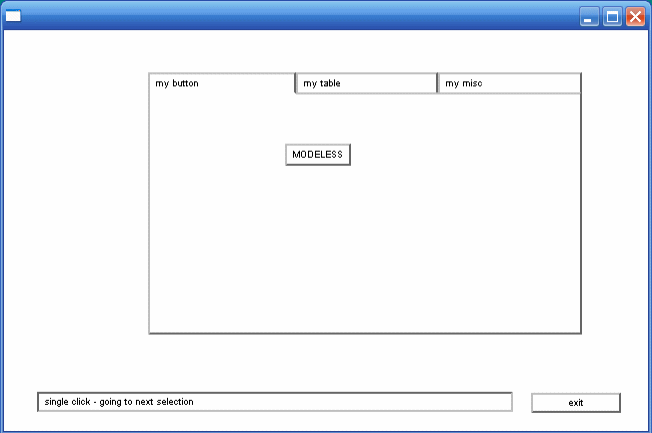
\includegraphics[width=0.9\linewidth]{assets/utr6/modeless.png}
\end{figure}


Figure 6: main.icn my button Tab


\textbf{Add a Message Box Label} to the canvas by clicking on the Label component (Abc) on the Ivib menu bar. Move the label to the bottom of the canvas and resize it to be almost the width of the canvas. Refer to the Figure 6. The message label is the long rectangle at the bottom of main.icn. Right Click on the Label to add some attributes as follows:


| On the \textbf{Other} tab, check the: | Class variable checkbox


Click the \textbf{Draw Border} check box so that there IS a border.


| On the \textbf{Name} tab enter: | Name label\_msgbox


| On \textbf{General} Tab enter: | Label : (make it blank - this label will be our message box) Hit Okay


From the Menu, Slect File->Save As and enter main.icn

\begin{Verbatim}[fontsize=\small,frame=single,commandchars=\\\{\}]
File->Save as:    main.icn
\end{Verbatim}


Make sure you save them in the directory you made for this application.


\textbf{Create an Edit Dialog} by going to the Ivib menu to File->New. A blank canvas will appear.


\textbf{Enter the canvas attributes}. Either right click on the Canvas for Dialog or go to the file menu option: Canvas->Dialog prefs.


| On the \textbf{Code} tab enter: | Name dialogedit


On the \textbf{Methods} tab, \textbf{un}-check the \texttt{Generate~main()~procedure} checkbox, so the checkbox is NOT checked. We DO NOT want to put a main procedure in this file.


On the \textbf{Attribs} tab, hit Add and replace Edit me with:

\begin{Verbatim}[fontsize=\small,frame=single,commandchars=\\\{\}]
Attrib      Value
label       Edit dialog     Hit Apply
font        sans,12     Hit Apply
\end{Verbatim}


This will add a title to the top of the canvas and change the default font to sans. You can also add different background and foreground colors by using the attributes bg and fg.


| On the \textbf{Events} Tab : | Hit Add and scroll down to \texttt{CLOSE\_BUTTON\_EVENT}. Enter on\_dialogedit   for the Event Handler and hit Apply. We will use this method to   capture the Windows X (close) Event at the top right of the Dialog.   Note Ivib may have added another event handler. Please delete it. The   CLOSE\_BUTTON\_EVENT handled by the on\_dialogedit method should be the   only entry. Hit Okay to close Dialog Prefs.


Add an Exit Button by clicking on the Button icon on the Tool Bar. Right Click on the Button to add some attributes as follows:


On the \textbf{General} tab enter:

\begin{Verbatim}[fontsize=\small,frame=single,commandchars=\\\{\}]
Label  Exit
\end{Verbatim}


On the \textbf{Name} tab enter:

\begin{Verbatim}[fontsize=\small,frame=single,commandchars=\\\{\}]
Name text_button_exit
\end{Verbatim}


On the \textbf{Other} tab check the:

\begin{Verbatim}[fontsize=\small,frame=single,commandchars=\\\{\}]
Class variable checkbox
\end{Verbatim}


| On the \textbf{Events} Tab, hit the Add Button. | Under Event: Scroll down to \texttt{BUTTON\_RELEASE\_EVENT}


| Under Handler enter: | \texttt{on\_text\_button\_exit} (it may be automatically added)


| Hit \textbf{Apply}. | Hit \textbf{Okay}


You may need to resize the button so the text will fit. Move the Exit button to bottom right corner as shown in Figure 7 of edit.icn below:

\begin{figure}[htbp]
\centering
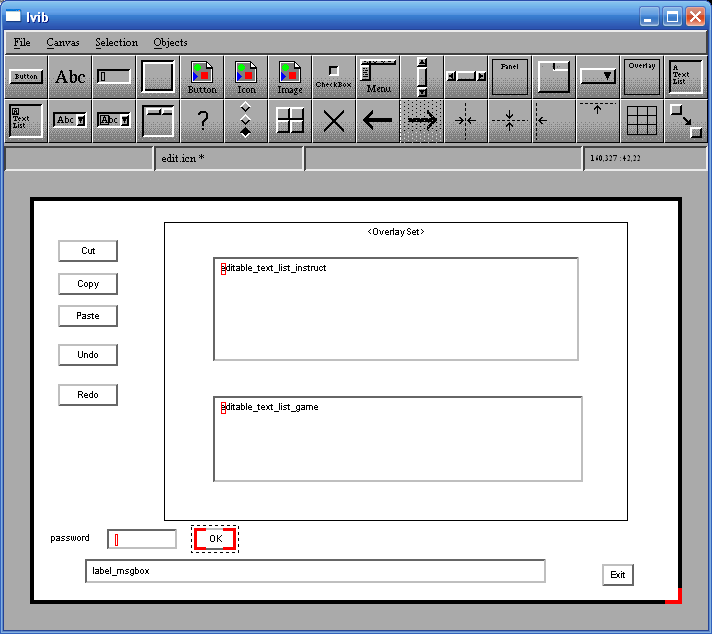
\includegraphics[width=0.9\linewidth]{assets/utr6/editicn.png}
\end{figure}


Figure 7: edit.icn


\textbf{Add a Message Box Label} to the canvas by clicking on the Label component (Abc) on the Ivib menu bar. Move the label to the bottom of the canvas and resize it to be almost the width of the canvas. Refer to Figure 7 of edit.icn. The message label is the long rectangle at the bottom of figure 7. Right click on the Label to add some attributes as follows:


| On the \textbf{Other} tab check the: | \textbf{Class variable} checkbox


Click the \textbf{Draw Border} check box so that there is a border.


| On the \textbf{Name} tab enter: | Name label\_msgbox


| On \textbf{General} tab enter: | Label : (make it blank - this label will be our message box) | Hit \textbf{Okay}


From Ivib, go to the File menu and execute this command:

\begin{Verbatim}[fontsize=\small,frame=single,commandchars=\\\{\}]
File->Save as:    edit.icn
\end{Verbatim}


Make sure you save them in the directory you made for this application and close Ivib.

\begin{enumerate}
\item 
Using an editor, open up main.icn
\end{enumerate}

\textbf{Caution!} Because you are saving files using Ivib and your editor, make sure that you save your file using the text editor before changing the graphics using Ivib. Also, make sure that you refresh the buffer (get the the latest) in your text editor after you change the graphics using Ivib. If you are nervous about writing over your changes you can make a backup copy to see how this works. Using the Gnu Emacs editor is a good idea, since it reminds you to refresh the buffer if Ivib has changed anything. Also, if you renamed any variables, the old names and their methods may still be there. Note: all variables are case sensitive so CancelBtn is not the same as cancelbtn. For example, if you forgot to uncheck \texttt{generate~main~procedure}, the main procedure will still remain. You will need to manually remove the main procedure and uncheck it in Ivib.


Edit main.icn and add the following code to the on\_text\_button\_modeless method:

\begin{Verbatim}[fontsize=\small,frame=single,commandchars=\\\{\}]

method on_text_button_modeless(ev)
  dedit := dialogedit()                   
  dedit.show_modeless()             # show edit dialog
  dispatcher.message_loop(dialogmain())
end
\end{Verbatim}


The third line \texttt{dispatcher.message\_loop(dialogmain())} makes the modal dialogmain the parent of the modeless dialogedit. When using modeless dialogs, at least one dialog must be modal. In this case, it is the main dialog. You only need to add this line once. If you call a modeless dialog from dedit, the dialogedit, you will not need this line.


Also, add \texttt{dispose()} to the \texttt{on\_text\_button\_exit()} method to close the dialog.

\begin{Verbatim}[fontsize=\small,frame=single,commandchars=\\\{\}]

method on_text_button_exit(ev)
  dispose()
end
\end{Verbatim}


Add the following code to on\_dialogmain so the dialog will close for the X event

\begin{Verbatim}[fontsize=\small,frame=single,commandchars=\\\{\}]

method on_dialogmain(ev)
  if \\ev.param = -11 then  #windows x box
     on_text_button_exit(ev)
end 
\end{Verbatim}


Save main.icn.


\textbf{Edit edit.icn} and add the following code to \texttt{on\_text\_button\_exit()} to close the dialog.

\begin{Verbatim}[fontsize=\small,frame=single,commandchars=\\\{\}]

method on_text_button_exit(ev)
   dispose()
end
\end{Verbatim}


Also add the following code to on\_dialogedit.

\begin{Verbatim}[fontsize=\small,frame=single,commandchars=\\\{\}]

method on_dialogedit(ev)
  if \\ev.param = -11 then  #windows x box
     on_text_button_exit(ev)
end
\end{Verbatim}


Save edit.icn.


Compile the program:

\begin{Verbatim}[fontsize=\small,frame=single,commandchars=\\\{\}]
> unicon -o demo -G main.icn edit.icn
\end{Verbatim}


Run the program

\begin{Verbatim}[fontsize=\small,frame=single,commandchars=\\\{\}]
> demo
\end{Verbatim}


When the main dialog comes up, you can click on the 'Modeless' button and a new edit dialog will appear. Notice you can go back and forth from main dialog to edit dialogs. Every time you click, a new dialog will be created. This is different from the show\_modal dialogs where the focus was only given to one dialog at a time.


We may not want our users creating too many dialog boxes. Let's add Some code to limit them to one only. If they click on the modeless button, and there is already a dialog open, we will set the focus on the already opened dialog box.


\textbf{In main.icn}, add the global variable dedit at the top of main.icn (before the class declaration). This is the edit dialog variable that will tell us if the dialog is open.

\begin{Verbatim}[fontsize=\small,frame=single,commandchars=\\\{\}]
global dedit
\end{Verbatim}


Add the following code to the \texttt{on\_text\_button\_modeless()} method and the \texttt{int\_dialog()} method.

\begin{Verbatim}[fontsize=\small,frame=single,commandchars=\\\{\}]

method on_text_button_modeless(ev)
   local winedit

   if \\dedit then \{
      if winedit := dedit.get_win() then \{
         Raise(winedit)
         dedit.set_focus(dedit.label_msgbox)
         return
      \}
   \}

   dedit := dialogedit()                   
   dedit.show_modeless()             # show edit dialog
   dispatcher.message_loop(dialogmain())
end
method init_dialog()
   dedit := &null
end
\end{Verbatim}


Save main.icn in the correct directory. In edit.icn, add the dedit := \&null line to the on\_text\_button\_exit method:

\begin{Verbatim}[fontsize=\small,frame=single,commandchars=\\\{\}]

method on_text_button_exit(ev)
    dedit := &null
    dispose()
 end
\end{Verbatim}


This sets the global variable \texttt{dedit} to \texttt{\&null} when the Dialog is closed. It can be closed by hitting the exit button or by hitting the X button in the right top corner.


Save the file. Compile and run the program. You will get only one edit dialog no matter how many times you hit the modeless button.

\subsubsection{Tables and Tabs Sets}
\label{utr6-tables-and-tabs-sets}

\textbf{Do not be confused!} Tables with a capital T are GUI components that arrange elements into rows and columns; they are not the same thing as the \texttt{table} data type.


\textbf{Add a Tabset to the main.icn canvas} by clicking on the Tabset Component from the Ivib Tool bar. It is the fourth component from the right on the top row. Move the Tabset to somewhere around the middle of the canvas. Enlarge it so it is similar to Figure 6. Right Click on the TabSet to add some attributes as follows:


On the \textbf{Other} tab check the: Class Variable checkbox


On the \textbf{Name} Tab enter: Name tab\_set\_demo


On the \textbf{General} tab you see: tab\_item\_1\textbackslash{}*


Click on it and an Edit box will appear. Change it as follows to create a tab for the button:

\begin{Verbatim}[fontsize=\small,frame=single,commandchars=\\\{\}]
Label: My button
Name: tab_item_btn
\end{Verbatim}


Hit \textbf{Apply}.


Now create another tab for a table by hitting Add and tab\_item\_2 will be added and highlighted. Change it as follows to create a tab for the Table:

\begin{Verbatim}[fontsize=\small,frame=single,commandchars=\\\{\}]
Label: My Table
Name: tab_item_table
\end{Verbatim}


\textbf{Class variable} should be checked. Hit \textbf{Apply}.


Now create a third tab by hitting Add and tab\_item\_3 will be added and highlighted. Change it as follows to create a tab for the Table:

\begin{Verbatim}[fontsize=\small,frame=single,commandchars=\\\{\}]
Label  My misc
Name: tab_item_misc
\end{Verbatim}


Hit \textbf{Apply}.


Hit Okay and the dialog box will close. You will need to enlarge horizontally the dialog so that the three tabs appear in order. Refer to Figure 6.


Move the modeless button from the main canvas to the my button tab.


Right click on the Tabset to open the Tabset Setup dialog box. At the bottom, on the General Tab, you see:

\begin{Verbatim}[fontsize=\small,frame=single,commandchars=\\\{\}]
tab_item_btn*
tab_item_table
tab_item_misc
\end{Verbatim}


The \texttt{*} after \texttt{tab\_item\_btn} indicates it is the tab item, you are currently editing. Click on tab\_item\_table so it is highlighted, then hit the which button. Now \texttt{tab\_item\_table} should have the star. Hit Okay, and you will now see on the main dialog that the \texttt{tab\_item\_table} tab can be edited.


Add a table to this tab, by clicking on the Table Component on the Ivib Tool Bar. It is the fourth component from the left in the bottom row. Move the table from the main canvas to the my table tab. Resize it as shown in the Figure 8 of main.icn below:

\begin{figure}[htbp]
\centering
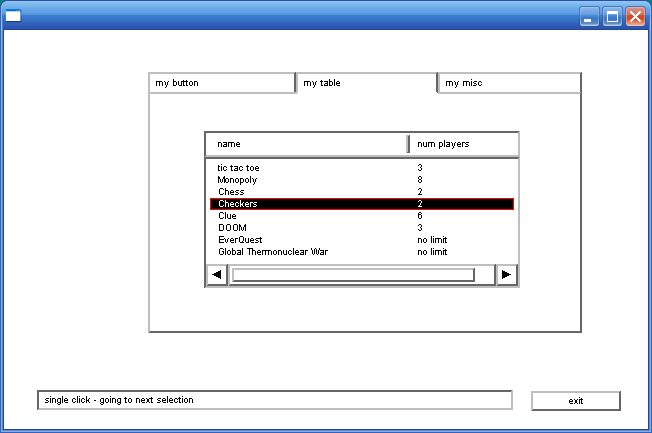
\includegraphics[width=0.9\linewidth]{assets/utr6/mainicn.png}
\end{figure}


Figure 8: main.icn


We are going to add some columns in the table so \textbf{right click on the table} to get the Table Setup Dialog.


On the \textbf{Other} tab check the: \textbf{Class Variable} checkbox.


On the \textbf{General} tab in Table Setup, Hit the Add button.


Now we will add the first column to our information table. Add the following to the \textbf{General} tab:

\begin{Verbatim}[fontsize=\small,frame=single,commandchars=\\\{\}]

Label :Name
Width: 200
Align l
Name: table_column_1 (class variable should be checked)
\end{Verbatim}


Hit Apply


Add another column by clicking the \textbf{Add} button:

\begin{Verbatim}[fontsize=\small,frame=single,commandchars=\\\{\}]

Label :# of Players
Width: 125
Align  l
Name: table_column_2
(class variable should be checked)
\end{Verbatim}


Hit \textbf{Apply}


On the \textbf{Selection} tab, the drop down box that says No selection, change this to \textbf{Select One}. Note: If you change it to Select Many, then they can select multiple rows by Control Shift and Click (mouse) at the same time.


On the \textbf{Events} tab, hit the Add Button.


| Under Event: Scroll down to \texttt{MOUSE\_RELEASE\_EVENT} | Under Handler enter: \texttt{on\_table\_1} (it may be automatically added)


Hit Apply


This will create a method \texttt{on\_table\_1()} that will be invoked by a \texttt{MOUSE\_RELEASE\_EVENT}. Note: Make sure that this is the only event added. Sometimes Ivib initially adds an \texttt{ACTION\_EVENT}. Please delete all other events.


Click \textbf{Okay} to close the setup dialog. You will probably need to make the Tabset and the Table larger as shown in Figure 8.


From the Ivib Menu, Save As \texttt{main.icn}.


Add the following code to the \texttt{init\_dialog()} method in \texttt{main.icn}:

\begin{Verbatim}[fontsize=\small,frame=single,commandchars=\\\{\}]

method init_dialog()
   local lst
   lst := [["tic tac toe","3"], ["Monopoly","8"], ["Chess","2"], ["Checkers","2"],
             ["Clue","6"],["DOOM","3"],["EverQuest","no limit"],["Global Thermonuclear War","no limit"]]
   table_1.set_contents(lst)
   dedit := &null
end
\end{Verbatim}


Save main.icn. Compile and run the program. You should be able to click on the tabs to display the three different tabs. Notice the 'My table Tab' is displayed first. We can change this by setting the \textbf{Which} back to \texttt{tab\_item\_btn} in Ivib if we want the button tab to show initially.

\subsubsection{Capturing Events, Click Counts and GoTo}
\label{utr6-capturing-events-click-counts-and-goto}

We are now going to add code so that an edit dialog box will come up every time we double click on one of the games in the table. We will add a global variable editdlg that is a table of dialogs. The keys for the table are the positions in the table. This example will demonstrate:

\begin{enumerate}
\item 
Double Click
\item 
Finding the selected positions and the contents of the table using \texttt{get\_contents()} and \texttt{get\_selections()}
\item 
Setting the position of the table by using set\_selections and go\_to.
\item 
Using Events to capture the right click and the Windows X close.
\end{enumerate}

Add the following global variable to \texttt{main.icn}. This is the table that will keep track of all the dialogs

\begin{Verbatim}[fontsize=\small,frame=single,commandchars=\\\{\}]
global editdlg
\end{Verbatim}


Also, add two more lines to the \texttt{init\_dialog()} method. The first new line initializes and creates the table \texttt{editdlg}. The second new line sets the click delay so we can distinguish double clicks from single clicks.

\begin{Verbatim}[fontsize=\small,frame=single,commandchars=\\\{\}]

method init_dialog()
local lst
   lst := [["tic tac toe","3"], ["Monopoly","8"], ["Chess","2"], ["Checkers","2"], ["Clue","6"],["DOOM","3"],["EverQuest","no limit"],["Global Thermonuclear War","no limit"]]
   table_1.set_contents(lst)
   dedit := &null
   editdlg := table()
   set_double_click_delay(100000)  # set click  delay  ford double click
end
\end{Verbatim}


Add the following code to the method \texttt{on\_table\_1()}:

\begin{Verbatim}[fontsize=\small,frame=single,commandchars=\\\{\}]

method on_table_1(ev)
local posn,poslst,msg,gamelst,cc
poslst := []
posn := 0
game := ""
gamelst := []
cc := 0

if \\ev & \\ev.source  & \\ev.type &  \\ev.param then 
   write("sc ",image(ev.source)," type ",image(ev.type)," param ",image(ev.param))
else
    return

if \\ev.param = -6 then \{ #right click
       posn := table_1.get_table_content().get_line_under_pointer() | 0
       if posn < 1 then return

       table_1.set_selections([posn]) #  add to selected list, highlight it
       table_1.goto_pos(posn)   
       table_1.set_cursor(posn)
       label_msgbox.set_label("right click demo at pos  "||posn)
       self.display()
       return
 \}
# 
#  returns list of selected items in this case only one because 'select one' is set for the table
  poslst :=  table_1.get_selections() | [] 
   if *poslst > 0 then
     posn := poslst[1]   # the selected position
   else
     return    
#  returns a list of lists with 2 items game and number players   
   gamelst :=  table_1.get_contents()  

#  get the selected name of the game from the table, the first item in the list
   game := gamelst[posn][1]
    cc := get_click_count()
   if cc > 1 then \{
       game := game || " double click "
#    create a global table editdlg to keep track of all the open dialogs  
     if not member (editdlg, posn) then \{
       (editdlg[posn] := dialogedit(posn,game))
       editdlg[posn].show_modeless()
     \}
     else \{
       Raise(editdlg[posn].get_win())
        editdlg[posn].set_focus(editdlg[posn].label_msgbox) 
     \}
     return

   \}  # end cc > 1

   if posn >= *gamelst then
       posn := 1
    else
       posn +:= 1

    table_1.set_selections([posn]) #  add to selected list, highlight it
    table_1.goto_pos(posn)   
    table_1.set_cursor(posn)
    label_msgbox.set_label("single click - going to next selection ")
    label_msgbox.display()
 end
\end{Verbatim}


Save main.icn.


First, this code will write the ev.param, ev.type and ev.code to determine what the ev.param is for a right click. It is -6, so if there is a right click, it is displayed in label\_msgbox and the selected position is highlighted and returns out of the method. Second, this code gets the selected item from a list of selected items by calling get\_selections. Since we have set the table in Ivib to `select one', only one item may be selected. So the list is either a one item list or empty if nothing has been selected. We can get the table contents by calling get\_contents. For tables, it will return a list of lists where each list (inside the big list) represents a row of size equal to the number of columns. In this example, we only have two columns; games and players. If an item is double clicked, then the edit dialog for the selected game and position is displayed.


This example also demonstrates the use of the goto\_pos, set\_cursor and set\_selections methods. If an item is single clicked, then the selection is moved to the next position unless it is the last position. If it is the last position, then it is moved to the first position. This is a pretty stupid thing to do, but it does demonstrate these features.


We are also passing the game name and its position to the edit dialog. So two variables will need to be added to the class definition for dialogedit in edit.icn as follows:

\begin{Verbatim}[fontsize=\small,frame=single,commandchars=\\\{\}]

class dialogedit : Dialog(posn, msg, label_msgbox, text_button_exit)
\end{Verbatim}


Note: Add posn as the first and msg as the second. The order is important. Also, note that Ivib will not alter them, but it will add new components in front of them. This means that you must move them back to the beginning if you add new components using Ivib.


Since we now have more multiple dialogs, we need to make sure they are set to \&null when the edit dialog terminates. Therefore, the following code will also need to be added to edit.icn.

\begin{Verbatim}[fontsize=\small,frame=single,commandchars=\\\{\}]

method init_dialog()
if \\msg & \\posn then
  label_msgbox.set_label(posn||" "||msg)
end
\end{Verbatim}


   method  on\_text\_button\_exit(ev)       delete(editdlg,posn)       dedit := \&null       dispose()    end


Save edit.icn. Compile and run the program. If you right click on any of the rows in the table, 'right click demo at position x' will be displayed in the message label. If you double click on any of the games, you will see either a new dialog or an existing dialog will be raised to the front. The new dialog will display the chosen game and it's position. If you single click, the cursor position goes to the next game or to the beginning if you are on the last game. This program also writes to standard output the values of ev.source, ev.type, and ev.param every time the mouse is released on the table.

\subsubsection{Overlays, and Hour Glasses}
\label{utr6-overlays-and-hour-glasses}

Open up edit.icn using Ivib. Add an Overlay to the edit.icn canvas, by clicking on the Overlay Component from the Ivib Tool Bar. It is the second component from the right in the top row. Move the Overlay to somewhere around the middle of the canvas. Enlarge it so its width and length are about twice the default size (see figure 7 of edit.icn). The overlay works very much like the Tabset component. It allows the program to hide components.


Right Click on the Overlay to add some attributes as follows:


On the \textbf{Other} tab, check the \textbf{Class Variable} checkbox.


On the \textbf{Name} tab, enter:

\begin{Verbatim}[fontsize=\small,frame=single,commandchars=\\\{\}]
Name overlay_set
\end{Verbatim}


| On the \textbf{General} tab, you see: | overlay\_item\_1\textbackslash{}*


Click on it and an Edit box will appear. Change the name as follows: This will be the initial overlay

\begin{Verbatim}[fontsize=\small,frame=single,commandchars=\\\{\}]
Name: overlay_item_blank
\end{Verbatim}


Hit Apply.


Create a second overlay by hitting \textbf{Add} and \texttt{overlay\_item\_2} will be added and highlighted. Change the name as follows:

\begin{Verbatim}[fontsize=\small,frame=single,commandchars=\\\{\}]
Name: overlay_item_edit
Hit Apply.
\end{Verbatim}


Click on \textbf{overlay\_item\_edit} so it is highlighted, then hit the \textbf{which} button. Now \textbf{overlay\_item\_edit} should have the star.


Hit \textbf{Okay} to close the setup dialog.


\textbf{Add an EditableText List Box} to the overlay by clicking the \textbf{EditableText List} component from the Ivib Menu Bar. It is the first one from the left in the second row. Move it on top of the Overlay and resize it (see figure 7 of edit.icn). Now, right click on it to get the dialog attributes.


On the \textbf{Other} tab, check the: \textbf{Class Variable} checkbox.


On the \textbf{Name} tab, enter:

\begin{Verbatim}[fontsize=\small,frame=single,commandchars=\\\{\}]
Name editable_text_list_instruct
\end{Verbatim}


Hit \textbf{Okay}.


\textbf{Add another EditableText List Box} to the overlay by clicking the \textbf{EditableText List} component from the Ivib Menu Bar. It is the first one from the left in the second row. Move it on top of the Overlay and move it directly under the editable\_text\_list\_instruct editabletextlist. (see figure 7 of edit.icn) Now, right click on it to get the dialog attributes


On the \textbf{Other} tab, check the \textbf{Class Variable} checkbox.


On the \textbf{Name} tab, enter:

\begin{Verbatim}[fontsize=\small,frame=single,commandchars=\\\{\}]
Name editable_text_list_game
\end{Verbatim}


Hit \textbf{Okay}.


Set the overlay back to the blank overlay by right clicking on the Overlay to change the which. At the bottom in the OverlaySet Setup panel, Click on \textbf{overlay\_item\_blank} so it is highlighted, then hit the \textbf{which} button. Now \textbf{overlay\_item\_blank} should have the star. Hit Okay.

\subsubsection{Copy, Cut, Paste, Undo and Redo}
\label{utr6-copy-cut-paste-undo-and-redo}

\textbf{Add 6 Buttons}. Move the buttons to the left of the overlay set (see figure 7 of edit.icn). Right Click on each the Buttons to add some attributes as follows:


On the \textbf{Other} tab, check: \textbf{Class Variable}


On the \textbf{Name} tab, enter: Name text\_button\_cut


On the \textbf{General} tab, enter: Label Cut


On the Events Tab add:

\begin{Verbatim}[fontsize=\small,frame=single,commandchars=\\\{\}]
Event                   Handler
BUTTON_RELEASE_EVENT            on_text_button_cut
\end{Verbatim}


\textbf{Make SURE this is the ONLY event. Delete any other events that may have been added by Ivib.}


\textbf{Hit Apply. Hit Okay.}


Do the same for the remaining buttons as follows:

\begin{Verbatim}[fontsize=\small,frame=single,commandchars=\\\{\}]
Name text_button_copy
Label  Copy
Name text_button_paste
Label  Paste
Name text_button_undo
Label  Undo
Name text_button_redo
Label  Redo
Name text_button_ok
Label  OK
\end{Verbatim}


We are going to create code to add and verify the password. First \textbf{Add a label} to the canvas by clicking on the Label component (Abc) on the Ivib menu bar. Move the label below the buttons (see figure 7 of edit.icn). Right Click on the Label to add some attributes as follows:


On the \textbf{Name} tab, enter: \texttt{Name:~label\_pw}


On \textbf{General Setup}: \texttt{Label~:~Password}


On the \textbf{Other} tab, check the \textbf{Class Variable} checkbox.


Hit \textbf{Okay}.


\textbf{Add a textfield} to the canvas by clicking on the textField component on the Ivib tool bar. This is the component third from the top left. Move the textfield below the buttons and just to the right of the label\_pw (see figure 7 of edit.icn). You may need to resize it. Right Click on the textfield to add some attributes as follows:


On the \textbf{Other} tab, check \textbf{Class Variable}


On the \textbf{Name Tab} enter: \textbf{Name text\_field\_pw}


Hit \textbf{Okay}.


You will probably want to resize it. Refer to Figure 7 of edit.icn. Save the Dialog in Ivib as \texttt{edit.icn}.


Now edit the source file \texttt{edit.icn}. Remember to refresh the Ivib changes.


Notice that in the class declaration, the components: \texttt{text\_button\_copy}, \texttt{text\_button\_cut}, \texttt{text\_button\_paste}, \texttt{text\_button\_redo}, \texttt{text\_button\_undo}, \texttt{text\_button\_ok}, \texttt{editable\_text\_list\_instruct}, \texttt{editable\_text\_list\_game}, \texttt{overlay\_set}, \texttt{text\_field\_pw} have been added before \texttt{posn} and \texttt{msg}. You will need to move them to the end because we are passing \texttt{posn} and \texttt{msg} from the main dialog, and they must be the first and second variable.


The class variables should look something like this when you are finished:

\begin{Verbatim}[fontsize=\small,frame=single,commandchars=\\\{\}]

class dialogedit : Dialog(posn, msg, text_button_copy, text_button_cut,
   text_button_paste, text_button_redo, text_button_undo, text_button_ok,
   editable_text_list_instruct, editable_text_list_game, overlay_set,
   text_field_pw , text_button_exit, label_msgbox, overlay_item_blank,
   overlay_item_edit, label_pw .............    )
\end{Verbatim}


We are going to let the user enter the game instructions only if they type in the password and hit the OK button. The overlay is initially set to \texttt{overlay\_item\_blank} because we set the which button in Ivib. However, when the correct password is typed, then the overlay will switch over to \texttt{overlay\_item\_edit} so the instructions can be entered. If the wrong password is typed and the OK button is hit, then we will make the user wait. This demonstrates the use of the hour glass mouse pointer. (Although, usually we use the hourglass when the program is processing). Add the following code to edit.icn as follows:

\begin{Verbatim}[fontsize=\small,frame=single,commandchars=\\\{\}]

method init_dialog()
if \\msg & \\posn then \{
   label_msgbox.set_label(posn||" "||msg)
   editable_text_list_game.set_contents([msg]) 
\}
text_field_pw.set_displaychar("*") # replace characters with * in password
end

method on_button_ok(ev)
local pw, t2, wait
pw := ""
label_msgbox.set_label("")
label_msgbox.display()

pw :=  text_field_pw.get_contents()
if pw == "joshua" then \{
     overlay_set.set_which_one(overlay_item_edit)
     label_msgbox.set_label("Enter Game Instructions ")
     label_msgbox.display()

\}
else \{
   t2 := &time  
   WAttrib(win,"pointer=" || ("wait"|"watch"))  # change mouse pointer to hourglass
   label_msgbox.set_label("Incorrect Password Please wait ")
   while &time - t2  < 5000 do 
        wait := 1
   WAttrib(win,"pointer=arrow")  # change mouse pointer to arrow
   label_msgbox.set_label("OK try again ")
   label_msgbox.display()

  \}
end
\end{Verbatim}


Save edit.icn. Compile and run the program. Double click on a game to get to the edit screen. You will see that if you type in the correct password ('joshua'), and hit Ok, the blank edit box where you can type in instructions will be visible. Hard coding passwords is not a good idea, but this example demonstrates the use of overlays and replacing the characters with stars. If you type in the wrong password, you will have to wait.


Open up edit.icn using your editor. Add the following code to the \texttt{init\_dialog()} method:

\begin{Verbatim}[fontsize=\small,frame=single,commandchars=\\\{\}]

method init_dialog()
 text_button_copy.clear_accepts_focus()  # keeps selected region 
 text_button_cut.clear_accepts_focus()    
  ........
  .........
end
\end{Verbatim}


NOTE: THIS CODE IS NECESSARY TO ALLOW THE SELECTED REGION IN THE EDITABLE TEXTLIST TO REMAIN SELECTED. OTHERWISE, THE SELECTED REGION WILL BE LOST WHEN THE EVENT OF HITTING THE COPY OR CUT BUTTON IS INVOKED.


Now add the following code for copy, cut, paste, redo and undo.

\begin{Verbatim}[fontsize=\small,frame=single,commandchars=\\\{\}]

method on_button_cut(ev)
editable_text_list_instruct.handle_cut()
end
method on_button_copy(ev)
editable_text_list_instruct.handle_copy()
end
method on_button_paste(ev)
editable_text_list_instruct.handle_paste()
end
method on_button_undo(ev)
editable_text_list_instruct.handle_undo()
end
method on_button_redo(ev)
editable_text_list_instruct.handle_redo()
end
\end{Verbatim}


Save edit.icn and compile and run the program.

\begin{Verbatim}[fontsize=\small,frame=single,commandchars=\\\{\}]
unicon -o demo -G main edit myeditabletextlist
\end{Verbatim}


You should be able to copy/cut/paste/undo/redo in the \texttt{editable\_text\_list\_instruct} box. However, you may want to copy text from other sources. We need to be able to cut/copy and paste using the Windows clipboard. To do this we will need to create a subclass for our EditableTextList. We will create a new file myeditabletextlist.icn that will inherit all the methods of editabletext list except for:

\begin{Verbatim}[fontsize=\small,frame=single,commandchars=\\\{\}]
handle_copy
handle_paste
handle_cut
\end{Verbatim}


Create a new file myeditabletextlist.icn and copy in the following code:

\begin{Verbatim}[fontsize=\small,frame=single,commandchars=\\\{\}]

#
# myeditabletextlist subclass of EditableTextList to 
# allow clipboard operation in Cut/Copy?paste
#
import gui
link graphics
import undo
$include "guih.icn"

class myeditabletextlist : EditableTextList()

   method handle_cut(e)
      start_handle(e)
      if has_region() then \{
         copy_to_clipboard(get_region())
         delete_region(e)
      \}
      end_handle(e)
   end

   method handle_copy(e)
      start_handle(e)
      if has_region() then \{
         copy_to_clipboard(get_region())
      \}
      end_handle(e)
   end

  method copy_to_clipboard(l)
   local large_str, i

   if /l | *l = 0 then fail
   large_str := l[1]

    every i := 2 to *l do
        large_str ||:=  l[i]

    WAttrib("selection=" || large_str)     
    return large_str

   end

   method get_list_from_clipboard()
   local large_str, l, str,start,blank1,tab1,p
   blank1 := ' '
   tab1 := '\\t'
   start := 1
   end1 := 1
   str := ""
   p := 1
   large_str := ""
   large_str := WAttrib("selection")
   if /large_str then fail
   l := []

   while   end1  :=   upto("\\n",large_str,start,0) do \{
      str := large_str[start:end1]
      if p := upto(&ascii--blank1,str) then
         str := str[p:0]
       put(l, str)
      start := end1 + 1
  \}
  str := large_str[start:0]
  if p := upto(&ascii--blank1--tab1,str) then
     str := str[p:0]
  put(l,str)

  return l
  end

#  insert_cr is a global variable to tell paste
#  to add a line feed after each line 
   method get_pasteable_clipboard(insert_cr)
      local x, t, s, c
      x := []
      t := ""

      x :=  get_list_from_clipboard() | fail

       every j := 1 to *x do  t := t || trim(string(x[j]))  || " "

      # Apply the filter to the string to paste
      s := ""
      every c := !t do \{
         if member(printable, c) then
            s ||:= c
      \}
      if *s = 0 then
         fail
      return s
   end

   method handle_paste(e,insert_cr)
      local s, ce, ed

      start_handle(e)
      if s := get_pasteable_clipboard(insert_cr) then \{
         ce := CompoundEdit()

         if has_region() then \{
            ed := EditableTextListDeleteRegionEdit(self)
            ed.redo()
            ce.add_edit(ed)
         \}
         ed := EditableTextListPasteEdit(self, s)
         ed.redo()
         ce.add_edit(ed)

         undo_manager.add_edit(ce)
         changed := 1
      \}
      end_handle(e)
   end
 end # myeditabletextlist class
\end{Verbatim}


Now open up edit.icn using Ivib. Right click on the Overlay set and switch to overlay\_item\_edit. Right click on the top edit box text\_list\_instruct to get the dialog box.


| On the \textbf{Name} tab, change the \textbf{Class} to \texttt{myeditabletextList}. | (Make sure this is all in lower case to match the class in   myeditabletextlist.icn)


Hit \textbf{Okay}, and save edit.icn


This will allow all cut/copy/pastes into \texttt{editable\_text\_list\_instruct} to use our subclass to pick up the windows clipboard.

\begin{Verbatim}[fontsize=\small,frame=single,commandchars=\\\{\}]
unicon -o demo -G main edit myeditabletextlist
\end{Verbatim}


Now, when you run demo you should be able to cut, copy, paste from other documents into the instructions edit box (editable\_text\_list\_instruct).

\subsubsection{Tab Jumps and Compound Undo/Redos}
\label{utr6-tab-jumps-and-compound-undo-redos}

There are a few more things we will add to the demonstration:

\begin{enumerate}
\item 
Tab Jumps
\item 
Compound Undos/Redos
\item 
Using events on table columns
\end{enumerate}

\textbf{Tab Jumps}. Open up edit.icn using your editor. Be sure to refresh to the changes from Ivib from above. Add the following code to the \texttt{init\_dialog()} method:

\begin{Verbatim}[fontsize=\small,frame=single,commandchars=\\\{\}]

method init_dialog()
editable_text_list_game.clear_accepts_focus() # allows tab jump or disables tab insert

 .......
 ........
end
\end{Verbatim}


NOTE: This code will not allow the tab to jump to the editable\_text\_list\_game box. It will disable any type of input to it. After completing this Tutorial, you may want to make editable\_text\_list\_game a 'myeditabletextlist' component so you can use the tabs, copy, cut, paste, undo, redo from the buttons. This will require that events are used to determine which edit box (editable\_text\_list\_game or editable\_text\_list\_list) to apply the function.


You may want to use the tab key to jump from one component to another. In our demo, the tab key just inserts a tab into the first text box in edit.icn. Suppose, we would like the tab key to jump to another component. To do this, you need to add the following methods to the subclass myeditabletextlist.icn:

\begin{Verbatim}[fontsize=\small,frame=single,commandchars=\\\{\}]

method keeps(e)
   # This component keeps all events.
   return e ~=== "\\t"
end

method handle_event(e)

   if (e === "\\t")  then 
      return

   (\\self.vsb).handle_event(e)
   (\\self.hsb).handle_event(e)
   if e === (&lpress | &rpress | &mpress) then
      handle_press(e)
   else if e === (&ldrag | &rdrag | &mdrag) then
      handle_drag(e)
   else if e === (&lrelease | &rrelease | &mrelease) then
      handle_release(e)
   else if \\self.has_focus then \{
      case e of \{
         Key_Home : handle_key_home(e)
         Key_End : handle_key_end(e)
         Key_PgUp : handle_key_page_up(e)
         Key_PgDn : handle_key_page_down(e)
         Key_Up : handle_key_up(e)
         Key_Down : handle_key_down(e)
         Key_Left : handle_key_left(e)
         Key_Right : handle_key_right(e)
         "\\b" : handle_delete_left(e)
         "\\r" | "\\l": handle_return(e)
         "\\^k" : handle_delete_line(e)
         "\\^a" : handle_select_all(e)
         "\\^e" : handle_end_of_line(e)
         "\\d" | "\\^d" : handle_delete_right(e)
         "\\^x" :  handle_cut(e)
         "\\^c" :  handle_copy(e)
         "\\^v" :  handle_paste(e)
         "\\^z" :  handle_undo(e)
         "\\^y" :  handle_redo(e)
         default : handle_default(e)
      \}
   \}
end
\end{Verbatim}


Compile and run the program. Notice that the tab key makes the cursor jump from component to component. If you want to order the tab jumps, go into Ivib, hit control-shift and simultaneously select the text\_button\_paste, text\_button\_undo, text\_button\_redo,text\_field\_pw, text\_button\_ok, text\_button\_exit in that order respectively. While still holding the control-shift, go to the Selection Item on the menu and select 'Reorder'. Now you can tab jump from top to bottom.

\subsubsection{Compound Undos and Redos}
\label{utr6-compound-undos-and-redos}

If you use undo and redo in our demo dialog, you will notice that the Undo undoes compound edits instead of single edits. If you would like to undo single edits, you will need to create a subclass of the undomanager. Create a file \texttt{myundomanager.icn} and copy the following code in to it.

\begin{Verbatim}[fontsize=\small,frame=single,commandchars=\\\{\}]

import undo
# UndoManager is a CompoundEdit.  Until it is closed it allows undos and redos
# within its list of edits, moving a pointer into the list appropriately.
#
class myundomanager:UndoManager(limit, index)
   method add_edit(other)
      if \\closed then
         return self.CompoundEdit.add_edit(other)
      while *l >= index do
          pull(l)
       put(l, other)
       index +:= 1

      while (*l > limit) & (index > 1) do \{
         index -:= 1
         pop(l)
      \}
   end
end # class
\end{Verbatim}


Now, edit \texttt{myeditabletextlist.icn}, and add initially code to use \texttt{MyUndoManager}. Add this code right before the class end statement:

\begin{Verbatim}[fontsize=\small,frame=single,commandchars=\\\{\}]

initially(a[])
   wordlist := []
   noedit := 0
   tab_move := &null
   self.LineBasedScrollArea.initially()
   self.set_accepts_focus()
   undo_manager := myundomanager()  # use local undomanager
   printable := cset(&cset[33:0]) ++ '\\t\\n'
   tab_width := 8
   set_wrap_mode("off")
   self.cursor_x := self.cursor_y := 1
   set_fields(a)   # insert initially before class end statement
# NO END STATEMENT FOR INITIALLY
\end{Verbatim}


    end \# class myeditabletextlist.icn


Compile and link

\begin{Verbatim}[fontsize=\small,frame=single,commandchars=\\\{\}]
unicon -o demo -G main edit  myeditabletextlist  myundomanager
\end{Verbatim}


Run the demo again to test the single undos/redos.

\subsubsection{Table Column Events}
\label{utr6-table-column-events}

So far we have just been using the table on the main screen to select the games (rows). We may also want to use the Name column or the \#Players column. In this example, we will sort the columns when a column is selected. The columns are actually components (subclasses of TextButton), and can be reached via the get\_column(n) method of Table, where n is the index of the column.


Edit main.icn. Add a class variable \texttt{table\_1\_col\_select} to the class declaration. We will use this variable to tell us if the column has been clicked. The class declaration should look like the following:

\begin{Verbatim}[fontsize=\small,frame=single,commandchars=\\\{\}]

class dialogmain : Dialog (table_1_col_select, tab_item_btn, ..........
\end{Verbatim}


Add the following lines to the end of \texttt{init\_dialog()}:

\begin{Verbatim}[fontsize=\small,frame=single,commandchars=\\\{\}]

method init_dialog()
   .......
   ......
   table_1_col_select := 0  # class variable initialize
   on_table_1()  # Listen for events
end
\end{Verbatim}


Next we need to add code to on\_table\_1 which is triggered by a MOUSE\_RELEASE\_EVENT to listen for a column event.


Add the following code to the beginning of the method on\_table\_1():

\begin{Verbatim}[fontsize=\small,frame=single,commandchars=\\\{\}]

method on_table_1(ev)
 local posn,poslst,msg,gamelst,cc
poslst := []
posn := 0
game := ""
gamelst := []
cc := 0
table_1.get_column(1).connect(self, "on_table_column_1", MOUSE_RELEASE_EVENT)
  if  table_1_col_select = 1 then \{
     table_1_col_select := 0 
     return
  \}

 table_1.get_column(2).connect(self, "on_table_column_2", MOUSE_RELEASE_EVENT)
  if  table_1_col_select = 1 then \{
     table_1_col_select := 0 
     return
  \}

if \\ev & \\ev.source  & \\ev.type &  \\ev.param then  
.......
........

end
\end{Verbatim}


Add the following to methods to handle the events. These methods Sort the selected columns:

\begin{Verbatim}[fontsize=\small,frame=single,commandchars=\\\{\}]

method on_table_column_1()
local lst,k,slst ,T
lst := []
slst := []
table_1_col_select := 1
lst :=    table_1.get_contents()
T := table()

every k := 1 to *lst do 
  insert(T,lst[k][1],lst[k][2])

lst := sort(T,1)
table_1.set_contents(lst) # sort by table key
end

method on_table_column_2()
local lst,k,slst ,T
lst := []
table_1_col_select := 1
lst :=    table_1.get_contents()
T := table()
every k := 1 to *lst do 
  insert(T,lst[k][1],lst[k][2])

lst := []
lst := sort(T,2)  # sort by table elements
table_1.set_contents(lst)
end
\end{Verbatim}


Compile and run. When you click on the table columns, they should sort by Name or number of players. This demonstrates the use of table columns.

\subsubsection{Conclusions and Future Work}
\label{utr6-conclusions-and-future-work}

Using IVIB is easy, but becoming proficient with it requires some familiarization and a certain comfort level with object-oriented programming. We believe this GUI toolkit is easier to learn than most competing tools. We plan to merge traditional IDE code editing, compiling, and executing capabilities into Ivib in a future release.


It is possible to use Ivib with regular procedural code, and it would be easy to extend Ivib to call a procedure for each event. This would allow Icon programmers to benefit from the new GUI toolkit. We would be happy to see this added to Ivib.

\paragraph{Acknowledgements}
\label{utr6-acknowledgements}

Robert Parlett inspired and astonished us by writing a GUI library better than we could have hoped for, entirely on his own, as a volunteer effort. His work was done in Idol and porting it to run under Unicon allowed us to identify some bugs in the new compiler. We hope our work adds value to Robert's accomplishment. Phillip Thomas provided corrections to this manuscript.

\section{References}
\label{utr6-references}

Ralph Griswold, Clinton Jeffery, and Gregg Townsend, "Graphics Programming in Icon", Peer-to-Peer Communications, 1998.


C. Jeffery, S. Mohamed, R. Pereda, R. Parlett, "Programming with Unicon", unicon.sourceforge.net/ub/ub.pdf, 2001-2005.

\begin{figure}[htbp]
\centering
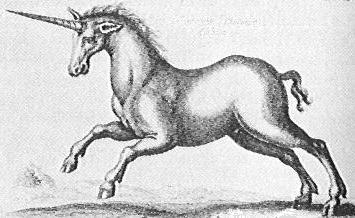
\includegraphics[width=0.9\linewidth]{assets/utr6/unilogo.jpg}
\end{figure}

\begin{figure}[htbp]
\centering
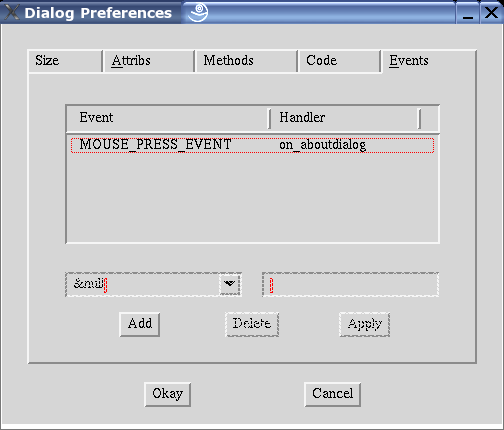
\includegraphics[width=0.9\linewidth]{assets/utr6/dlogpref.png}
\end{figure}

\end{document}
